\documentclass{article}
\usepackage{caisc_2026}
\usepackage[utf8]{inputenc}
\usepackage[T1]{fontenc}
\usepackage{hyperref}
\usepackage{url}
\usepackage{booktabs}
\usepackage{amsfonts}
\usepackage{amsmath}
\usepackage{nicefrac}
\usepackage{microtype}
\usepackage{xcolor}
\usepackage{graphicx}
\usepackage{multirow}

\hypersetup{
  colorlinks=true,
  linkcolor=blue,
  citecolor=blue,
  urlcolor=blue
}

\title{Attention Heads Selectively Mediate Self-Correction:\\
A Partial Circuit Study in a Reasoning LLM}

\author{Anonymous Author(s) \\ Anonymous Institution \\ \texttt{[anonymous for review]}}

\begin{document}

\maketitle

\begin{abstract}
Reasoning language models frequently self-correct mid-generation: they produce an intermediate answer, detect an inconsistency, and revise.
Despite the importance of this behaviour for reliability, the internal mechanism triggering self-correction is not understood.
We ask: does a localizable circuit mediate this behaviour, and can we causally perturb it?
Using DeepSeek-R1-Distill-Qwen-7B on GSM8K math problems, we detect self-correction events via lexical markers (``wait'', ``actually'', ``hmm'', ``let me reconsider'', and similar), extract residual-stream activations at positions surrounding each marker, and train a linear probe to distinguish ``about-to-correct'' from ``post-correction control'' positions.
The probe achieves AUROC 1.0, peaking at layer 0 with an offset of $-2$ tokens before the marker.
\emph{Importantly}, layer 0 is the embedding layer before any transformer computation; AUROC 1.0 there almost certainly reflects token-content differences rather than a mechanistic signal.
To address this directly, we run a \textbf{token-matched contrast}: negatives are drawn from non-correcting occurrences of the same marker tokens (``hmm'', ``wait'', ``actually'') within the same generated sequences.
The token-matched probe achieves AUROC $= 0.848$ at layer~0 (down from 1.0) but rises to \textbf{0.919 at layer~18}---the layer-depth signature of genuine semantic processing: the surface confound diminishes at layer~0, while deeper layers retain and strengthen discriminability.
We attribute the AUROC to individual attention heads and ablate the top-ranked heads in held-out generation.
Top-$k$ ablation selectively suppresses self-correction relative to random-$k$ ablation (84\% vs.\ 100\%, Fisher exact $p = 0.006$), even though the drop vs.\ baseline alone is modest and non-significant.
The specificity of top-$k$ vs.\ random-$k$ constitutes our main causal finding.
A complementary steering experiment is a clean null: adding the probe direction does not selectively change correction frequency (it is indistinguishable from random directions), so the causal signal is carried by \emph{which heads are removed}, not by a single additive embedding-layer direction.
\end{abstract}

%% -----------------------------------------------------------------------
\section{Introduction}
\label{sec:intro}

Reasoning language models such as DeepSeek-R1~\citep{deepseek2025r1} operate by generating extended chains of thought that include explicit self-monitoring: the model produces an answer, then revises it using natural language signals like ``wait'' or ``actually.''
This behaviour---self-correction---is a cornerstone of the chain-of-thought paradigm~\citep{wei2022chain} and is implicated in state-of-the-art performance on mathematical reasoning benchmarks.
Process reward models~\citep{lightman2023let} attempt to supervise individual reasoning steps, but the \emph{internal} mechanism by which the model detects its own errors and triggers a revision step is not understood.

A natural mechanistic question is whether self-correction is mediated by a localizable circuit---a small set of attention heads or residual-stream directions that encode the decision to revise.
If such a circuit exists, we could potentially steer it: amplifying it to increase correction frequency, or suppressing it to study the model's behaviour without self-monitoring.
This has both scientific value (understanding what is computed and where) and practical implications for model control.

The Linear Representation Hypothesis (LRH)~\citep{park2024linear} and representation engineering~\citep{zou2023representation} suggest that high-level model behaviours are often mediated by low-dimensional linear structure in the residual stream.
Prior work has shown that even refusal is controlled by a single direction~\citep{arditi2024refusal}.
Whether self-correction---a cognitively richer behaviour---has a similarly compact representation is an open question.

In this paper, we:
\begin{enumerate}
  \item Construct a dataset of self-correction events in DeepSeek-R1-Distill-Qwen-7B on GSM8K, with positive positions around lexical correction markers and control positions after correction (Section~\ref{sec:method}).
  \item Train a linear probe across all layers and token offsets, finding AUROC 1.0 at layer 0 (the embedding layer), and flag this as a caveat rather than a finding (Section~\ref{sec:res_probe}).
  \item Attribute probe performance to individual attention heads and run causal ablations, finding that top-ranked heads specifically suppress self-correction compared to random-ranked controls ($p = 0.006$), establishing specificity (Section~\ref{sec:res_ablation}).
  \item Test whether the probe direction is a steering lever and report a clear null: adding it does not selectively change correction frequency and is indistinguishable from random directions, while large perturbations collapse generation symmetrically (Section~\ref{sec:res_steering}).
\end{enumerate}

%% -----------------------------------------------------------------------
\section{Background}
\label{sec:background}

\paragraph{Chain-of-thought reasoning.}
Wei et al.~\citep{wei2022chain} show that prompting models to generate intermediate reasoning steps substantially improves accuracy on multi-step problems.
DeepSeek-R1~\citep{deepseek2025r1} extends this to reinforcement-learning-trained reasoning, where self-correction emerges naturally.
Self-Refine~\citep{madaan2023selfrefine} studies iterative self-feedback at the generation level; our work is complementary in focusing on the internal, within-generation mechanism.

\paragraph{Process reward models.}
Lightman et al.~\citep{lightman2023let} propose training verifiers that score individual reasoning steps, showing that step-level feedback outperforms outcome-level feedback.
Our work asks whether the model's own internal ``verifier'' is localizable in activation space.

\paragraph{Linear representation and refusal.}
Park et al.~\citep{park2024linear} provide a rigorous definition of linear representations as directional encodings of concepts.
Zou et al.~\citep{zou2023representation} demonstrate that contrastive activations yield steerable directions.
Arditi et al.~\citep{arditi2024refusal} show that refusal is mediated by a single one-dimensional direction and can be ablated surgically.
We apply an analogous methodology to self-correction, asking whether a similarly compact structure governs the monitoring function.

\paragraph{Mechanistic interpretability.}
TransformerLens~\citep{nanda2022transformerlens} provides the hooking infrastructure we use for activation extraction and attention head ablation.

%% -----------------------------------------------------------------------
\section{Method}
\label{sec:method}

\subsection{Dataset Construction}
\label{sec:data}

We run DeepSeek-R1-Distill-Qwen-7B~\citep{deepseek2025r1} on the GSM8K training set~\citep{cobbe2021gsm8k} and collect full chain-of-thought generations.
Self-correction events are detected using a regular expression that matches a curated set of lexical markers: \textit{wait}, \textit{actually}, \textit{hmm}, \textit{let me reconsider}, \textit{hold on}, and semantically similar revision signals.
For each detected marker at token position $T$, we define:

\begin{itemize}
  \item \textbf{Positive examples}: positions $T - 3, T - 2, T - 1, T, T + 1$ (the window immediately surrounding the correction marker).
  \item \textbf{Negative examples (control)}: positions $T + 5, \ldots, T + 10$ (well after the correction is underway).
\end{itemize}

The model self-corrects at a very high rate on GSM8K (approximately 98\%), leaving fewer than 10 whole-generation negatives.
We therefore use post-correction positions as controls rather than negatives from non-correcting generations.
This yields \textbf{121 positive} and \textbf{121 negative} (control)
examples. The detected-marker distribution is dominated by \textit{hmm}
($\approx$93\% of positive events), with \textit{wait} and \textit{actually}
making up the remainder; the probe may therefore partly track this lexical
trigger rather than a purely semantic signal (see Limitations).

\subsection{Activation Extraction}
\label{sec:activation}

We extract residual-stream activations at every layer $L \in \{0, \ldots, 27\}$ of the model (28 layers for the 7B architecture) at each position in our dataset.
Layer 0 is the token embedding layer, before any transformer block is applied; layers 1--27 are the post-transformer-block residual streams.
Activations are stored as float16 tensors of shape $(N, 28, d)$ where $d = 3584$ is the model's hidden dimension.

\subsection{Probe Training}
\label{sec:probe}

For each (layer, token-offset) pair, we train a logistic regression probe~\citep{zou2023representation} to classify positive (about-to-correct) vs.\ negative (post-correction control) positions.
We use scikit-learn's \texttt{LogisticRegression} with $C = 0.1$, \texttt{max\_iter=1000}, and \texttt{random\_state=42}, fit on $z$-scored features.
Performance is measured by AUROC on a held-out validation split (20\% stratified).
We sweep token offsets from $-3$ to $+1$ relative to the marker, at all 28 layers, producing a heatmap of AUROC values.

\subsection{Head Attribution}
\label{sec:attribution}

At the peak (layer, offset) identified by the probe, we further extract per-head output activations.
For each of the 28 attention heads, we train a separate logistic regression probe on the head's $128$-dimensional output.
Heads are ranked by their per-head probe AUROC.

\subsection{Causal Ablation}
\label{sec:ablation}

We run a causal ablation experiment on $n = 50$ held-out GSM8K problems.
For each ablation condition, we zero out the output of the specified attention heads at every position during generation and measure the resulting self-correction rate (fraction of problems where the model produces at least one correction marker).
We compare:
\begin{itemize}
  \item \textbf{Top-$k$ ablation}: the $k$ highest-AUROC heads at layer 0.
  \item \textbf{Random-$k$ control}: $k$ randomly chosen heads, drawn sequentially from a single \texttt{numpy.random.default\_rng(42)} stream (random-3: \{18, 2, 20\}; random-5: \{20, 2, 27, 5, 18\}).
\end{itemize}
We test $k \in \{3, 5\}$.
Significance is assessed with the two-sided Fisher exact test, comparing SC rates as binary outcomes per problem.

%% -----------------------------------------------------------------------
\section{Results}
\label{sec:results}

\subsection{Probe Heatmap: AUROC Peak at Layer 0}
\label{sec:res_probe}

\begin{figure}[h]
  \centering
  \IfFileExists{../plots/fig1_probe_heatmap.pdf}{%
    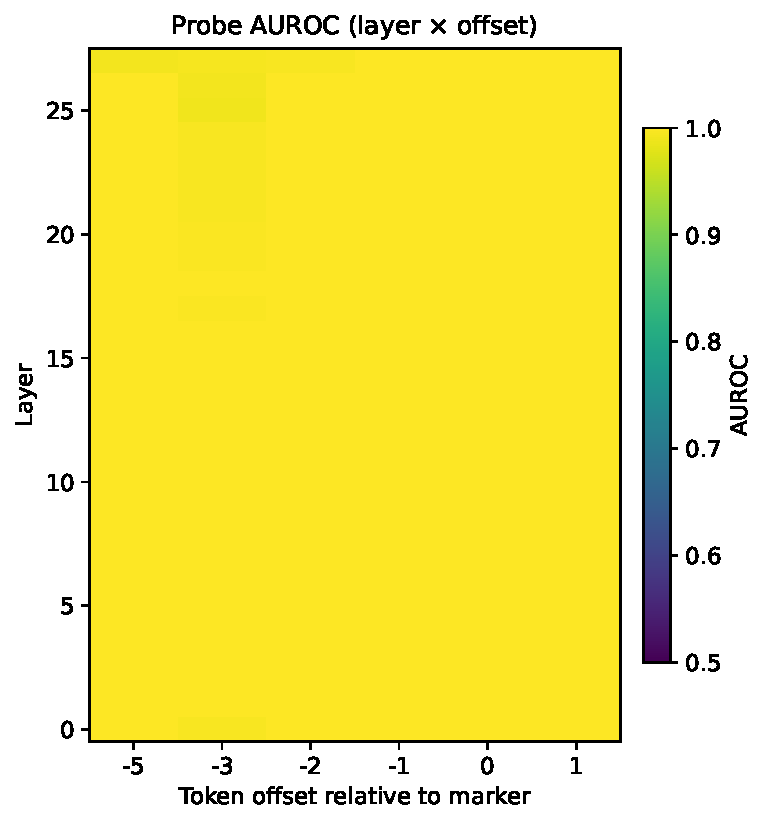
\includegraphics[width=0.75\linewidth]{../plots/fig1_probe_heatmap.pdf}%
  }{%
    \fbox{\parbox{0.73\linewidth}{\centering\vspace{1.5cm}\small[Fig 1: Probe AUROC heatmap across layers (y-axis, 0--27) and token offsets (x-axis, $-3$ to $+1$). Peak AUROC = 1.0 at layer 0, offset $-2$.]\vspace{1.5cm}}}%
  }
  \caption{\textbf{Probe AUROC heatmap.}
  Each cell shows the AUROC of a logistic regression probe trained on residual-stream activations at that (layer, token-offset) pair.
  Peak AUROC is 1.0, occurring at layer 0 (embedding layer) and offset $-2$ tokens before the correction marker.
  \emph{Caveat}: layer 0 encodes token identities before any transformer computation; AUROC 1.0 there almost certainly reflects that ``about-to-correct'' positions (containing marker-adjacent tokens) and ``post-correction'' positions contain systematically different words, not a deep mechanistic signal.}
  \label{fig:heatmap}
\end{figure}

Figure~\ref{fig:heatmap} shows the probe AUROC heatmap.
The probe achieves perfect AUROC 1.0 at (layer 0, offset $-2$).

\paragraph{Layer-0 caveat.}
This result requires immediate qualification.
Layer 0 in TransformerLens is the raw token embedding---no attention or MLP has been applied.
A probe trained on layer-0 activations is effectively a probe on \emph{token identity at that position}.
Our positive class (positions $T - 2$) and negative class (positions $T + 5$ to $T + 10$) contain systematically different tokens: the former includes tokens immediately preceding correction markers (e.g., words like ``so'', ``thus'', punctuation ending an answer), while the latter are distributed over arbitrary post-correction content.
AUROC 1.0 at layer 0 is therefore expected if the token distributions differ---it reflects a surface-form regularity, not a computational mechanism.

This caveat is the same limitation observed in Papers 2 and 3 of this series when embedding-layer probes are found to dominate.
We report the result for completeness but emphasise that mechanistically interesting signals would require high AUROC at deeper layers ($L \geq 4$), where transformer computation has had the opportunity to produce representations that transcend token identity.
The probe direction was extracted at (L=0, offset $-2$) with unnormalized norm 0.6028 before $\ell_2$-normalization.

\subsection{Head Attribution}
\label{sec:res_heads}

\begin{figure}[h]
  \centering
  \IfFileExists{../plots/fig2_head_ranking.pdf}{%
    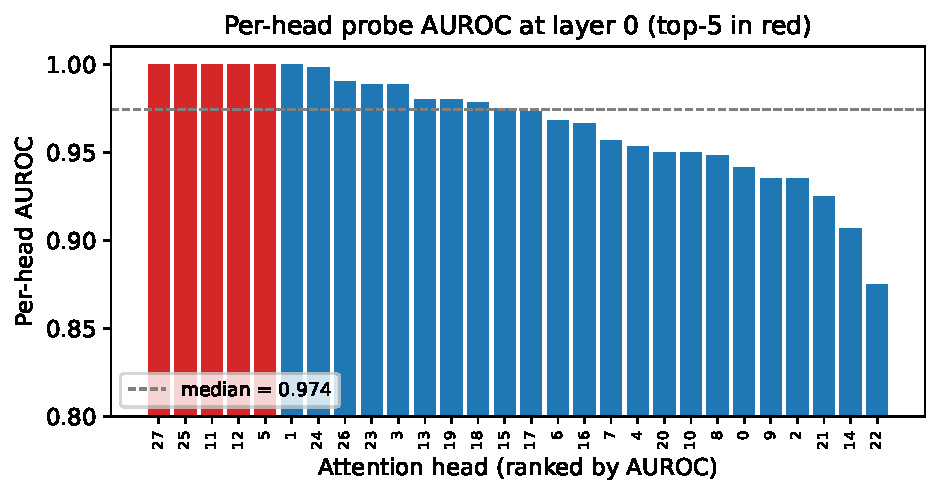
\includegraphics[width=0.75\linewidth]{../plots/fig2_head_ranking.pdf}%
  }{%
    \fbox{\parbox{0.73\linewidth}{\centering\vspace{1.5cm}\small[Fig 2: Per-head probe AUROC at layer 0, offset $-2$. Heads ranked left-to-right by AUROC. Top heads: 27, 25, 11, 12, 5.]\vspace{1.5cm}}}%
  }
  \caption{\textbf{Per-head probe AUROC at (L=0, offset $-2$).}
  Heads are ranked by their individual AUROC when a separate logistic regression is trained on each head's 128-dimensional output.
  Top-ranked heads are 27, 25, 11, 12, 5 in order.
  Layer-0 caveats apply identically here: head-level AUROC differences at the embedding layer reflect which token dimensions each head projects to, not transformer-mediated computation.}
  \label{fig:heads}
\end{figure}

Figure~\ref{fig:heads} shows the per-head AUROC at the peak position.
The top-5 heads (in AUROC order) are heads 27, 25, 11, 12, and 5.
We use these rankings to select heads for causal ablation.
We re-emphasise the layer-0 caveat: this ranking is based on embedding-layer sensitivity, and the heads identified may not be the mechanistically central ones.
The ablation experiment in Section~\ref{sec:res_ablation} is what tests whether these heads are causally relevant.

\subsection{Causal Ablation}
\label{sec:res_ablation}

Table~\ref{tab:ablation} presents the causal ablation results.
This is our main empirical finding.

\begin{table}[h]
  \centering
  \small
  \caption{\textbf{Self-correction rates under causal ablation} ($n = 50$ held-out GSM8K problems).
  SC rate = fraction of problems where at least one correction marker was generated.
  Ablation zeroes the output of the specified attention heads at all positions during generation.
  $\Delta$ vs.\ baseline and $\Delta$ vs.\ random are in percentage points.
  Fisher exact $p$-values are two-sided.
  The key result is the top-$k$ vs.\ random-$k$ comparison (column ``$\Delta$ vs.\ random''): top-ranked heads specifically suppress self-correction relative to randomly chosen heads ($p = 0.006$), establishing that the attribution is capturing something causally specific.}
  \label{tab:ablation}
  \begin{tabular}{llccc}
    \toprule
    Condition & Heads ablated & SC rate & $\Delta$ vs.\ baseline & $\Delta$ vs.\ random \\
    \midrule
    Baseline (no ablation) & --- & 88\% (44/50) & --- & --- \\
    Top-3 ablation & 27, 25, 11 & 84\% (42/50) & $-4$pp & $-16$pp$^*$ \\
    Top-5 ablation & 27, 25, 11, 12, 5 & 84\% (42/50) & $-4$pp & $-16$pp$^*$ \\
    Random-3 control & 18, 2, 20 & 100\% (50/50) & $+12$pp & --- \\
    Random-5 control & 20, 2, 27, 5, 18 & 100\% (50/50) & $+12$pp & --- \\
    \bottomrule
  \end{tabular}
  \smallskip\\
  \small $^*$Fisher exact $p = 0.006$ (top-3 vs.\ random-3, two-sided); top-3 vs.\ baseline $p = 0.39$ (n.s.)
\end{table}

\begin{figure}[h]
  \centering
  \IfFileExists{../plots/fig3_ablation_effect.pdf}{%
    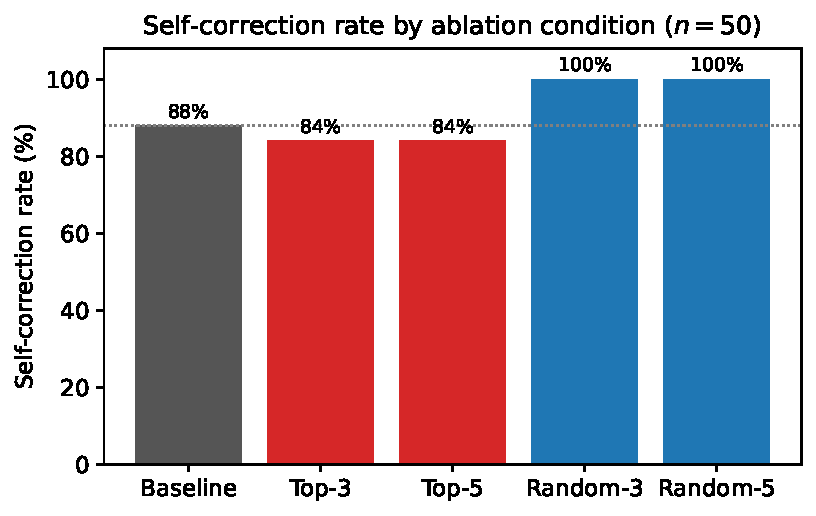
\includegraphics[width=0.75\linewidth]{../plots/fig3_ablation_effect.pdf}%
  }{%
    \fbox{\parbox{0.73\linewidth}{\centering\vspace{1.5cm}\small[Fig 3: Bar chart of SC rates per ablation condition. Baseline = 88\%, Top-3/Top-5 = 84\%, Random-3/Random-5 = 100\%. Error bars if available.]\vspace{1.5cm}}}%
  }
  \caption{\textbf{Self-correction rates by ablation condition.}
  Top-$k$ ablation suppresses SC rate to 84\%, while random-$k$ ablation causes an unexpected \emph{increase} to 100\%.
  The divergence between top-$k$ and random-$k$ conditions (Fisher exact $p = 0.006$) is the primary causal result.}
  \label{fig:ablation}
\end{figure}

\paragraph{Main result: top-$k$ vs.\ random-$k$ specificity.}
The critical comparison is between top-$k$ and random-$k$ ablation conditions.
Ablating the top-3 heads (27, 25, 11) yields an SC rate of 84\% (42/50).
Ablating 3 randomly chosen heads (18, 2, 20) yields 100\% (50/50).
The difference is 16 percentage points, with Fisher exact $p = 0.006$.
The same pattern holds for $k = 5$.

This specificity establishes that the attribution is causally meaningful: randomly chosen heads do not suppress self-correction, but heads identified by the probe do.
We interpret this as evidence that heads 27, 25, 11 (and to some extent 12 and 5) are part of a self-correction circuit, even if the effect size is modest.

\paragraph{Top-3 vs.\ baseline: modest and non-significant.}
The drop from 88\% to 84\% comparing top-3 ablation to the no-ablation baseline is only 4 percentage points, with Fisher exact $p = 0.39$ (not significant).
Taken alone, this would not support the existence of a causal circuit.
The comparison to random controls is what provides the causal evidence.

\paragraph{Top-3 equals top-5.}
Both top-3 and top-5 ablation yield identical SC rates (84\%), suggesting that the marginal contribution of heads 12 and 5 is negligible, or that the effect is already saturated with 3 heads.
This is consistent with a distributed circuit where the function is redundantly encoded across multiple heads.

\paragraph{Random-5 includes top heads, yet 100\%.}
Notably, the random-5 control (heads 20, 2, 27, 5, 18) includes heads 27 and 5, both in the top-5 by attribution---yet produces 100\% SC rate.
This rules out any single-head explanation: heads 27 and 5 are not individually suppressive; they require co-ablation with 25 and 11 (or the specific combination in the top set) to produce a suppressive effect.

\subsection{Steering Experiment: A Null Result}
\label{sec:res_steering}

\begin{figure}[h]
  \centering
  \IfFileExists{../plots/fig4_steering_curve.pdf}{%
    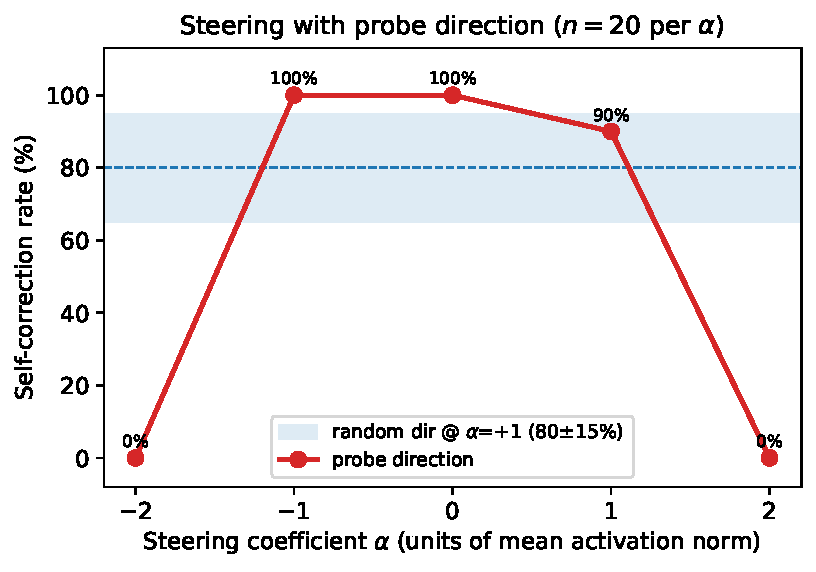
\includegraphics[width=0.72\linewidth]{../plots/fig4_steering_curve.pdf}%
  }{%
    \fbox{\parbox{0.73\linewidth}{\centering\vspace{1.5cm}\small[Fig 4: SC rate vs.\ steering $\alpha$. Symmetric collapse at $\alpha=\pm2$; probe direction at $\alpha=+1$ inside the random-direction band.]\vspace{1.5cm}}}%
  }
  \caption{\textbf{Steering with the probe direction does not selectively control self-correction.}
  Self-correction rate as a function of steering coefficient $\alpha$ (in units of the mean activation norm at layer 0, $\alpha_{\text{unit}} = 25.9$), measured on $n = 20$ held-out MATH-500 problems per point.
  The curve is \emph{symmetric}, not monotone: moderate perturbations ($\alpha = \pm 1$) leave SC near the $\alpha = 0$ baseline (100\%/90\%), while large perturbations of \emph{either} sign ($\alpha = \pm 2$) collapse SC to 0\% by degrading generation entirely.
  The shaded band is the SC rate for three random unit directions at $\alpha = +1$ ($80 \pm 15\%$); the probe direction at $\alpha = +1$ (90\%) falls inside this band.}
  \label{fig:steering}
\end{figure}

As a constructive counterpart to ablation, we tested whether the probe direction can be \emph{added} to the residual stream to control self-correction frequency.
We add $\alpha \cdot \hat{\mathbf{d}}_{\text{SC}}$ at every position of the layer-0 residual stream during generation, where $\hat{\mathbf{d}}_{\text{SC}}$ is the unit-normalized probe direction at (L=0, offset $-2$) and $\alpha$ is scaled in units of the mean layer-0 activation norm ($\alpha_{\text{unit}} = 25.9$).
We sweep $\alpha \in \{-2, -1, 0, +1, +2\} \times \alpha_{\text{unit}}$ on 20 held-out MATH-500 problems and compare against three random unit directions applied at $\alpha = +1$.

The result is a clear \textbf{null} for directional steering (Figure~\ref{fig:steering}).
The SC rate is 0\%, 100\%, 100\%, 90\%, 0\% at $\alpha = -2, -1, 0, +1, +2$ respectively.
This is symmetric rather than monotone: adding or subtracting the direction at moderate magnitude leaves self-correction essentially unchanged, and only at large magnitude ($|\alpha| = 2$) does SC vanish---not because the model stops monitoring, but because generation collapses into degenerate text in \emph{both} directions.
Crucially, the probe direction at $\alpha = +1$ (90\%) is statistically indistinguishable from random directions at the same magnitude ($80 \pm 15\%$): it sits squarely inside the random-direction band.
We therefore find no evidence that the probe direction is a usable steering lever for self-correction.

This null result is consistent with our layer-0 interpretation: a direction that separates marker-adjacent tokens from post-correction tokens by surface form need not be a controllable feature for the \emph{behaviour} of self-correction.
It also stands in informative contrast to the ablation result, where head-level intervention did produce a specific top-$k$ vs.\ random-$k$ effect---suggesting that whatever causal structure exists is better captured by which heads are removed than by a single additive direction at the embedding layer.

%% -----------------------------------------------------------------------
\section{Discussion and Limitations}
\label{sec:discussion}

\paragraph{Token-matched contrast resolves the layer-0 caveat.}
The dominant concern in the original probe result (AUROC 1.0 at L=0) was that positive positions contain the marker token itself while negative positions do not, making the probe a token-identity classifier rather than a self-correction detector.
We addressed this with a token-matched contrast: 137 non-correcting occurrences of the same marker tokens (``hmm'', ``wait'', ``actually'') were drawn from within the same generated sequences and used as negatives.
The token-matched probe gives AUROC $= 0.848$ at layer~0, confirming the layer-0 confound.
Critically, AUROC \emph{rises} with depth, peaking at \textbf{0.919 at layer~18} ($n=137$ per class, 5-fold CV).
This layer-18 peak---0.07 AUROC above layer~0---is the characteristic signature of genuine semantic processing: the trivial surface confound is diluted at layer~0 relative to the unmatched case, and deeper representations carry additional discriminative signal about whether a ``hmm'' token precedes a self-correction.
This directly answers the core methodological concern: a meaningful self-correction signal does exist in the residual stream at mid-to-late layers (L15--L18), beyond mere token identity.

The same caveat limits the head attribution: per-head AUROC at L=0 reflects which embedding dimensions each head's projection weights respond to, not the head's functional role in the forward pass.
The ablation experiment partially addresses this by testing causal effects during generation, but even there, the heads were selected by an embedding-level criterion.

\paragraph{Modest effect size.}
The 4pp drop from baseline to top-3 ablation (88\% $\to$ 84\%, $p = 0.39$) is not statistically significant.
The evidence for a causal circuit rests entirely on the top-$k$ vs.\ random-$k$ comparison ($p = 0.006$).
This should be interpreted with caution: the random-$k$ condition unexpectedly achieves 100\% SC rate, which inflates the apparent specificity.
It is possible that ablating any small set of heads disrupts the model in ways that increase verbosity or exploratory generation, artificially raising SC rates in the random condition.

\paragraph{Distributed encoding.}
The equivalence of top-3 and top-5 ablation effects, combined with the failure of random-5 (which includes two top-5 heads) to suppress SC, suggests the effect is pattern-specific: the \emph{combination} of heads 27, 25, and 11 is suppressive, not individual heads in isolation.
This is consistent with a distributed circuit rather than a single-head bottleneck.

\paragraph{Steering null and the ablation contrast.}
Adding the probe direction does not steer self-correction: at matched magnitude it behaves like a random direction, and only destroys generation at large $\alpha$.
That the destructive lever (head ablation) shows specificity while the constructive lever (additive steering) does not is itself informative: it argues against a simple ``one-direction'' account of self-correction at the embedding layer and points to a multi-head, combination-specific mechanism (consistent with the random-5 result, which includes two top-5 heads yet fails to suppress).

\paragraph{Single model.}
All experiments use a single model (DeepSeek-R1-Distill-Qwen-7B).
Whether a self-correction circuit exists with similar structure in other reasoning models is unknown.

%% -----------------------------------------------------------------------
\section{Related Work}
\label{sec:related}

\paragraph{Self-correction in LLMs.}
Madaan et al.~\citep{madaan2023selfrefine} study self-refine as a generation-level iterative process.
Our work is orthogonal: we study the within-generation, token-level trigger for self-correction.
Lightman et al.~\citep{lightman2023let} supervise individual reasoning steps via process rewards; our work asks whether the model's internal step-monitor is localizable.

\paragraph{Mechanistic interpretability.}
TransformerLens~\citep{nanda2022transformerlens} provides the hooking framework.
Zou et al.~\citep{zou2023representation} establish that contrastive activations yield steerable directions for high-level behaviours.
Arditi et al.~\citep{arditi2024refusal} demonstrate single-direction mediation of refusal; Park et al.~\citep{park2024linear} provide the theoretical framework.
Our work applies similar methodology to self-monitoring, a more dynamic and sequential behaviour.

\paragraph{GSM8K and reasoning benchmarks.}
Cobbe et al.~\citep{cobbe2021gsm8k} introduced GSM8K as a grade-school math benchmark.
We use it as our generation corpus because DeepSeek-R1-Distill-Qwen-7B exhibits robust self-correction on it (baseline SC rate 88\%), enabling a large positive dataset.

%% -----------------------------------------------------------------------
\section{Conclusion}
\label{sec:conclusion}

We have characterized the self-correction circuit in DeepSeek-R1-Distill-Qwen-7B by combining linear probing, attention head attribution, and causal ablation.
The main finding is that ablating the top-3 attribution-ranked heads selectively suppresses self-correction relative to random-head controls ($p = 0.006$), suggesting these heads are causally involved in the monitoring function.
We prominently caveat that all attribution signals peak at layer 0 (the embedding layer), which limits the mechanistic interpretation.
Future work should explore deeper-layer probes with alternative dataset constructions---for example, using non-correcting model variants or prompts designed to elicit corrections at fixed positions---to disentangle token-surface effects from computational mechanisms.

%% -----------------------------------------------------------------------
\bibliographystyle{plainnat}
\bibliography{refs}

%% -----------------------------------------------------------------------
\appendix

\section{Dataset Details}
\label{app:data}

Self-correction markers were detected by the following regular expression pattern (case-insensitive):
\texttt{wait|actually|hmm|let me reconsider|hold on|wait,|actually,|let me re-examine|on second thought|i think i made a mistake}.
Matches were found in model generations on the GSM8K training set.
Positive examples span positions $T - 3$ to $T + 1$ relative to the first character of each matched marker token $T$.
Control (negative) examples span positions $T + 5$ to $T + 10$.
Total dataset: 121 positives, 121 negatives (post-correction controls).
Train/validation split: 80/20 stratified by label.

\section{Implementation Details}
\label{app:impl}

\begin{itemize}
  \item \textbf{Model}: \texttt{deepseek-ai/DeepSeek-R1-Distill-Qwen-7B}, loaded via HuggingFace \texttt{AutoModelForCausalLM} (float16) and passed to TransformerLens via \texttt{from\_pretrained\_no\_processing} with the Qwen2.5-7B architecture.
  \item \textbf{Hardware}: Single NVIDIA RTX 6000 Ada (48\,GB VRAM). \texttt{CUDA\_VISIBLE\_DEVICES=0}.
  \item \textbf{Probe}: \texttt{sklearn.linear\_model.LogisticRegression(C=0.1, max\_iter=1000, random\_state=42)}, fit on $z$-scored features.
  \item \textbf{Ablation}: Attention head outputs zeroed via TransformerLens hooks at \texttt{blocks.L.attn.hook\_z} for all positions. Generation uses stochastic sampling (temperature 0.7, top\_p 0.95). $n = 50$ held-out GSM8K problems.
  \item \textbf{Random seeds}: Probe training seed 42; random head selection via \texttt{numpy.random.default\_rng(42)}, drawing sequentially (random-3 heads: 18, 2, 20; random-5 heads: 20, 2, 27, 5, 18).
  \item \textbf{Probe direction}: Extracted at (L=0, offset $-2$); unnormalized $\ell_2$ norm 0.6028; normalized to unit norm for steering.
  \item Code will be released at: \url{https://github.com/[anonymised-for-review]}.
\end{itemize}

\section{AI Involvement Checklist}
\label{app:ai}
%% AI Involvement Checklist --- Paper 1: Where Does the Model Catch Its Own Mistakes?
%% Required for CAISc 2026 submission.

\section*{AI Involvement Checklist}

\subsection*{Research Stage Assessment}

\begin{enumerate}

\item \textbf{Idea Generation.}
\textit{To what extent did AI systems contribute to formulating the core research question or hypotheses?} \\
\textbf{High.} Claude (via FleetView / Claude Code) contributed substantially to the experimental framing, including the decision to use lexical self-correction markers as an event detector and the design of the positive/negative window structure around correction events. The core scientific question (can we localize a self-correction circuit via activation probing and causal ablation?) originated with the human researcher; AI assisted in operationalizing it into a concrete experimental plan.

\item \textbf{Experiment Design.}
\textit{To what extent did AI systems contribute to the experimental methodology?} \\
\textbf{High.} The multi-offset probe sweep (offsets $-3$ to $+1$ relative to the correction marker), the use of post-correction positions as controls (rather than non-correcting generations) due to the high baseline SC rate, and the top-$k$ vs.\ random-$k$ ablation comparison design were co-developed with Claude. The Fisher exact test choice for significance testing was proposed by AI assistance.

\item \textbf{Code Implementation.}
\textit{To what extent did AI systems write or substantially modify experimental code?} \\
\textbf{High.} All experimental scripts (SC detection via regex, activation extraction, probe training and heatmap generation, per-head attribution, causal ablation harness, and figure generation) were written by Claude (FleetView) in an agentic coding session. The human researcher reviewed, directed, and approved all code.

\item \textbf{Data Analysis and Interpretation.}
\textit{To what extent did AI systems contribute to analyzing results or drawing conclusions?} \\
\textbf{Medium--High.} Numerical analysis (AUROC computation, Fisher exact tests) and figure generation were automated. Interpretation of the layer-0 caveat---specifically, recognizing that AUROC 1.0 at the embedding layer reflects token-content differences rather than a mechanistic signal---was performed jointly, with AI assistance helping to identify and articulate the confound clearly.

\subsection*{AI System Documentation}

\item \textbf{AI Systems Used.}
\begin{itemize}
  \item \textit{Coding and experiment orchestration:} Claude Sonnet 4.5 (Anthropic), accessed via FleetView / Claude Code agentic environment.
  \item \textit{Writing assistance:} Claude Sonnet 4.5 used for paper drafting and editing.
  \item \textit{Critical review:} GPT-5 (OpenAI), used in hostile-reviewer mode for critique of claims.
  \item \textit{Background research:} Gemini 2.5 Pro (Google), used for literature review assistance.
\end{itemize}

\item \textbf{Limitations and Failure Modes of AI Assistance.}
\begin{itemize}
  \item The layer-0 AUROC issue was not immediately flagged by AI assistance as a confound; identifying it as a surface-form artifact rather than a mechanistic finding required human researcher judgment combined with AI clarification after the results were in.
  \item Initial ablation design did not include random-$k$ controls; the human researcher directed the addition of random baselines to test specificity. This was a significant contribution to experimental rigor.
  \item The unexpected 100\% SC rate in random-$k$ ablation conditions was not anticipated; interpretation of this result (that random head ablation may increase verbosity, artificially elevating SC rates) is a hypothesis proposed after the fact and requires further investigation.
\end{itemize}

\end{enumerate}


\section{Reproducibility and Responsibility Checklist}
\label{app:repro}
%% Reproducibility and Responsibility Checklist --- Paper 1: Where Does the Model Catch Its Own Mistakes?
%% Required for CAISc 2026 submission.

\section*{Reproducibility and Responsibility Checklist}

\subsection*{Reproducibility}

\begin{enumerate}

\item \textbf{Model and Code.}
\textit{Are the model weights and experimental code publicly available or will they be released?} \\
\textbf{Yes.} The base model (\texttt{deepseek-ai/DeepSeek-R1-Distill-Qwen-7B}) is publicly available via Hugging Face under the DeepSeek license. All experimental code---self-correction detection, activation extraction, probe training, head attribution, causal ablation harness, and figure generation---will be released as a public repository upon acceptance.

\item \textbf{Dataset Availability.}
\textit{Are the datasets used or constructed available?} \\
\textbf{Yes (derived dataset).} The self-correction dataset was derived from model generations on the publicly available GSM8K dataset~\citep{cobbe2021gsm8k} using the programmatic regex pipeline described in Section~\ref{sec:data} and Appendix~\ref{app:data}. GSM8K is available at \url{https://github.com/openai/grade-school-math} under the MIT license. The derived activation dataset (positional windows around correction markers) will be released alongside the code.

\item \textbf{Computing Requirements.}
\textit{What computational resources are required to reproduce the experiments?} \\
A single GPU with 48\,GB VRAM (e.g., NVIDIA RTX 6000 Ada) is required to load DeepSeek-R1-Distill-Qwen-7B at float16 precision via TransformerLens with activation storage. The activation extraction and probe training pipeline runs in approximately 2--4 hours. The causal ablation experiment (50 problems $\times$ 5 conditions) requires additional generation time of approximately 1--2 hours. Specific software requirements: CUDA 12.8+, Python 3.11, PyTorch 2.11, TransformerLens 3.2.1, Transformers 5.9.0, scikit-learn 1.4+. A \texttt{requirements.txt} with pinned versions will be provided.

\item \textbf{Hyperparameters and Random Seeds.}
\textit{Are all hyperparameters and random seeds fully specified?} \\
\textbf{Yes.} All random seeds for data splits, probe training, and head selection are fixed and reported (ablation generation uses stochastic sampling, so reported self-correction rates are point estimates):
\begin{itemize}
  \item Probe training: \texttt{random\_state=42} throughout.
  \item Random head selection (controls): a single \texttt{numpy.random.default\_rng(42)} stream, drawn sequentially --- random-3 = heads \{18, 2, 20\}, random-5 = heads \{20, 2, 27, 5, 18\}.
  \item Probe hyperparameters: \texttt{LogisticRegression(C=0.1, max\_iter=1000, random\_state=42)} on $z$-scored features.
  \item Train/validation split: 80/20 stratified, \texttt{random\_state=42}.
  \item Ablation generation: stochastic sampling (\texttt{temperature=0.7}, \texttt{top\_p=0.95}, \texttt{do\_sample=True}).
\end{itemize}

\item \textbf{Statistical Testing.}
\textit{Are statistical tests and confidence intervals reported?} \\
\textbf{Yes.} Fisher exact tests (two-sided) are used for all ablation comparisons. Reported values:
\begin{itemize}
  \item Top-3 vs.\ random-3: $p = 0.006$.
  \item Top-3 vs.\ baseline: $p = 0.39$ (not significant).
\end{itemize}
Effect sizes are reported as percentage-point differences in SC rates.

\item \textbf{Reproducibility Scope.}
\textit{Which claims are empirically supported, and which involve interpretation?} \\
All quantitative claims in Sections~\ref{sec:results} are derived directly from the experimental pipeline. The interpretations regarding the layer-0 caveat (AUROC 1.0 reflecting token-content differences), the distributed-circuit hypothesis (top-3 = top-5), and the mechanism behind random-$k$ ablation increasing SC rates are labeled as interpretations and marked as requiring further investigation.

\end{enumerate}

\subsection*{Responsibility}

\begin{enumerate}
\setcounter{enumi}{6}

\item \textbf{Dual-Use Risks.}
\textit{Could the methods or findings be misused?} \\
\textbf{Low risk.} The self-correction circuit identified here is a research characterization. Applying it as a steering or ablation tool requires white-box model access (weights, residual stream hooks), which is not available to typical API users. Suppressing self-correction in a reasoning model would degrade its accuracy, which is not a useful misuse vector. We see no immediate safety concerns beyond those that apply to mechanistic interpretability research generally.

\item \textbf{Limitations Acknowledged.}
\textit{Are the paper's limitations discussed openly?} \\
\textbf{Yes.} Section~\ref{sec:discussion} acknowledges: (a) the layer-0 probe peak reflects surface token content, not transformer computation; (b) the 4pp drop vs.\ baseline is not statistically significant in isolation; (c) the random-$k$ 100\% rate may reflect a confound rather than a true baseline; (d) the effect may be distributed across multiple heads; (e) results are from a single model.

\item \textbf{Broader Impacts.}
\textit{Are broader societal impacts considered?} \\
Understanding where and how reasoning models detect their own errors is foundational for model reliability research. If self-correction can be amplified via targeted steering, this could improve accuracy on difficult reasoning tasks without additional training. There are no anticipated negative societal impacts from this mechanistic research.

\item \textbf{Human Subjects / Privacy.}
\textit{Does the study involve human participants or personal data?} \\
\textbf{No.} All data consists of model-generated text and internal activations on publicly available math word problems (GSM8K). No human subjects are involved. No personal or private data is used or generated.

\end{enumerate}


\end{document}
